\documentclass[12pt]{article}
\usepackage[letterpaper]{geometry}
\usepackage{amsmath, amsthm, amssymb, amsfonts}
\usepackage{graphicx}
\usepackage{titling}
\usepackage{hyperref}
\newcommand{\subtitle}[1]{%
  \posttitle{%
    \par\end{center}
    \begin{center}\large#1\end{center}
    \vskip0.5em}%
}
\hypersetup{
    colorlinks=true,
    linkcolor=blue,
    filecolor=magenta,      
    urlcolor=blue,
} 
\urlstyle{same}
\title{CSE 150 - Operating Systems \\ Documentation \#2}
\subtitle{Spring 2018 - Lab 04 - Group 1}
\author{Avery Berchek, Aleksandr Brodskiy, David Cabral, Christopher DeSoto,\\Adiam G-Egzabher, Nanditha Embar, Christian Vernikoff}
\begin{document}
\maketitle
{\setlength{\parindent}{0cm}
\textbf{Outline}
\begin{enumerate}  
\item Documentation
\item Design Decisions
\item Testing/QA
\item Design Questions
\item Team Member Work-Log
\item Conclusion\\\\\\\\\\\\\\\\
\end{enumerate} 
}
{\setlength{\parindent}{0cm}
\textbf{Documentation}\\
\begin{center}Task I\end{center}
The pseudo$-$code amounted thus far for the implementation of a user processes with the ability to access a file system through various 
\textsc{syscall}s is demonstrated below.
\begin{center}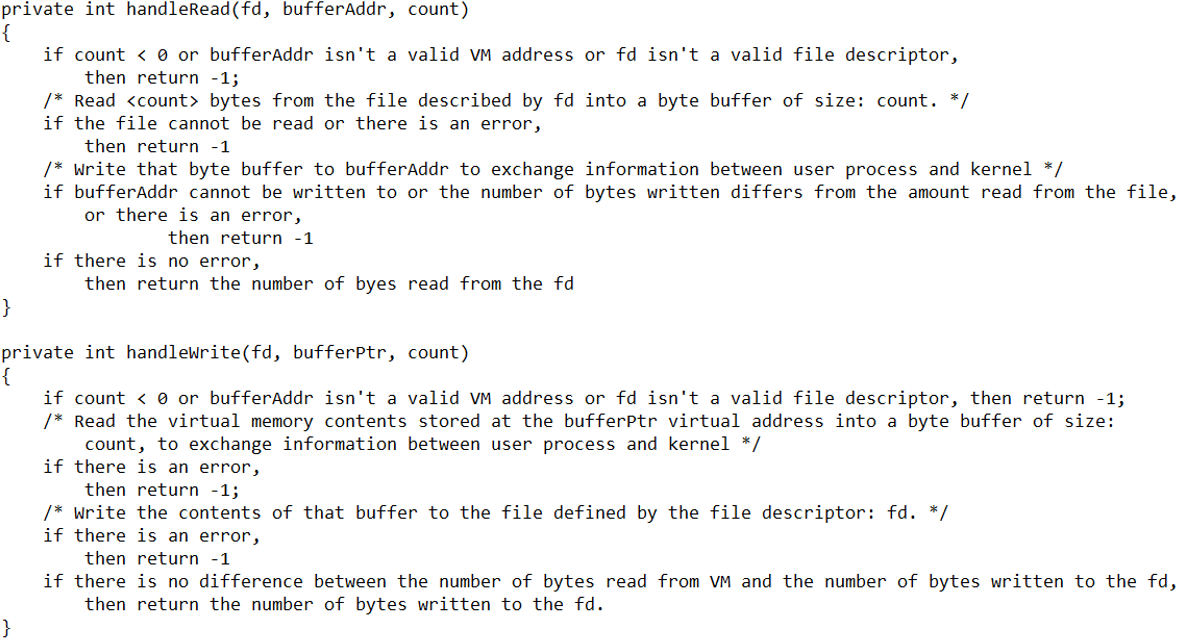
\includegraphics[width=150mm]{pic1_1.png}\end{center}
From the pseudo$-$code it is observable that the various \textsc{syscall}s are implemented through the handler functions which perform
 \textit{unlinkng}, \textit{creating}, \textit{opening}, \textit{writing}, \textit{reading}, \& \textit{closing} manipulations on the 
 respective \textsc{file}s and their corresponding memory addresses.
\begin{center}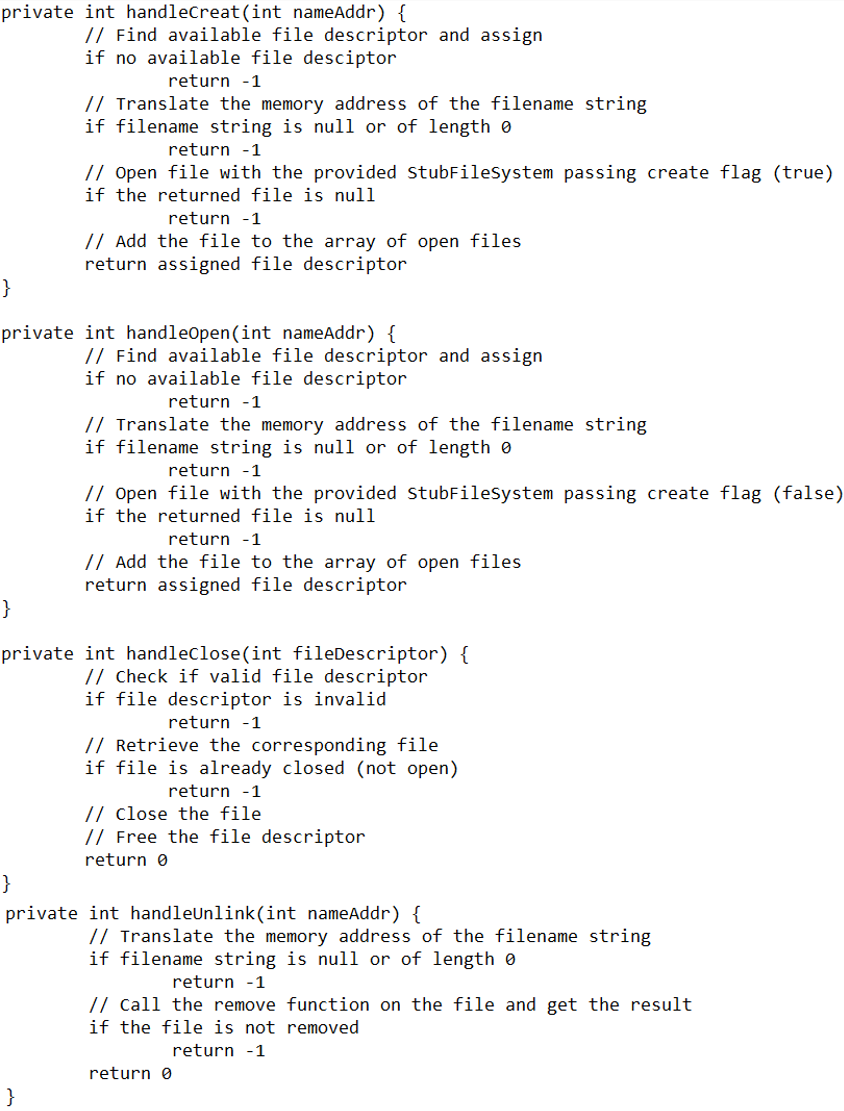
\includegraphics[width=130mm]{pic5.png}\end{center}
\paragraph{}It is observable that the six functions defined are the
 \textsc{handleRead}, \textsc{handleWrite}, \textsc{handleCreat}, \textsc{handleOpen}, \textsc{handleClose}, \& \textsc{handleUnlink}
 functions which enable user processes to manipulate \textsc{Read}able and \textsc{Write}able files, respectively. Within this manipulative capability are the underlining
 essentials of UNIX/POSIX functional system calls. As such, the control flow ensures that the provides with them the checks for validity of \textsc{file} \textit{descriptors}
 and \textsc{filename}s. \\ \paragraph{}In this manner the functionality of the implemented pseudo$-$code is relatively straightforward and essentially self$-$explanatory.  
\begin{center}Task II\end{center}
The initial implementation of user processes for the support of multi$-$programming paradigms is demonstrated below, through the following definitions 
of the \textsc{loadSection} and \textsc{read}/\textsc{write} pseudo$-$code functions to the \textit{pages} of \textit{virtual memory},
which were eventually changed to accommodate for certain discrepancies which will be reviewed in greater detail in the \textbf{Desing Decision} section.
\begin{center}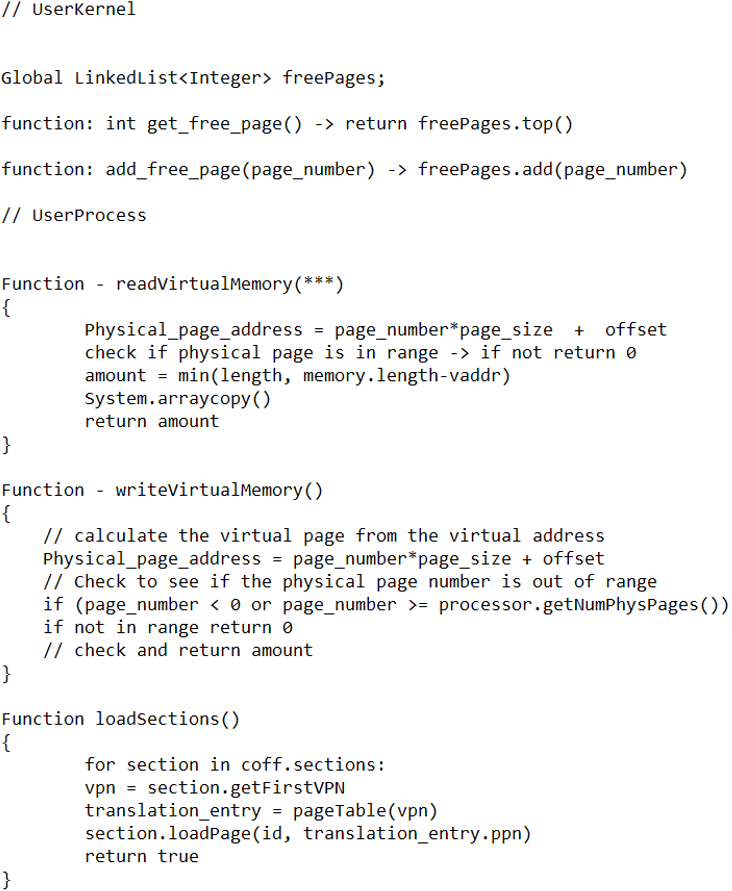
\includegraphics[width=100mm]{pic2.png}\end{center}
This implementation entails the maintenance of a global linked list of physical \textit{free}$-$pages for the allocation of memory by 
utilizing pages for new user processes. With the exclusion of the \textsc{loadSection} function however, the reformatted \textit{read} $\&$ \textit{write} functions have been amended
to ameliorate the handle reading and writing across page boundaries. The page boundary issue was mitigated with the utmost attention to potential error as the \textsc{read} $\&$ \textsc{write} \textsc{VirtualMemory} functions check that the Virtual address is indeed valid to avoid reading an erroneous and unnecessarily large buffer size.
This was done by setting the physical page address equal to the offset added to the product of the page number and the page size. 
\begin{center}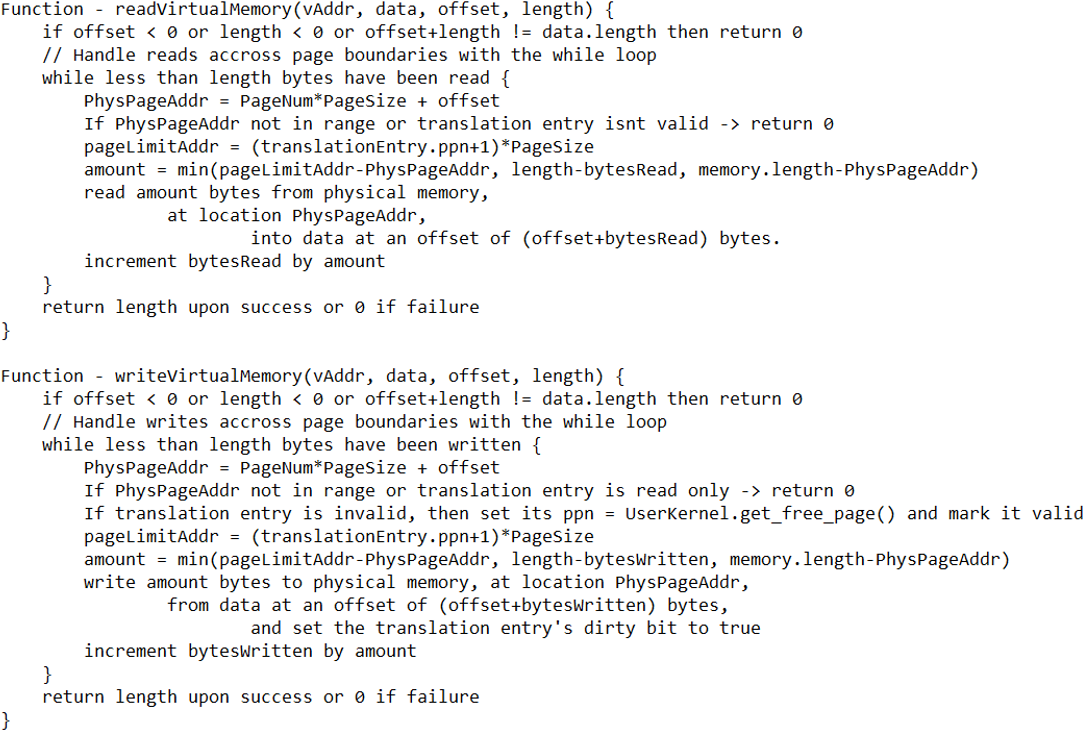
\includegraphics[width=150mm]{pic2_1.png}\end{center}
\begin{center}Task III\end{center}
The algorithmic functionality of the 
\begin{center}
\textsc{UserProcess.java} \\
\textsc{exit}, \textsc{exec}, \textsc{join} $\longrightarrow 1, 2, 3$ \\
\end{center}
The pseudo$-$code implementations of the \textsc{exit}, \textsc{exec}, and \textsc{join} system calls is demonstrated below:
\begin{center}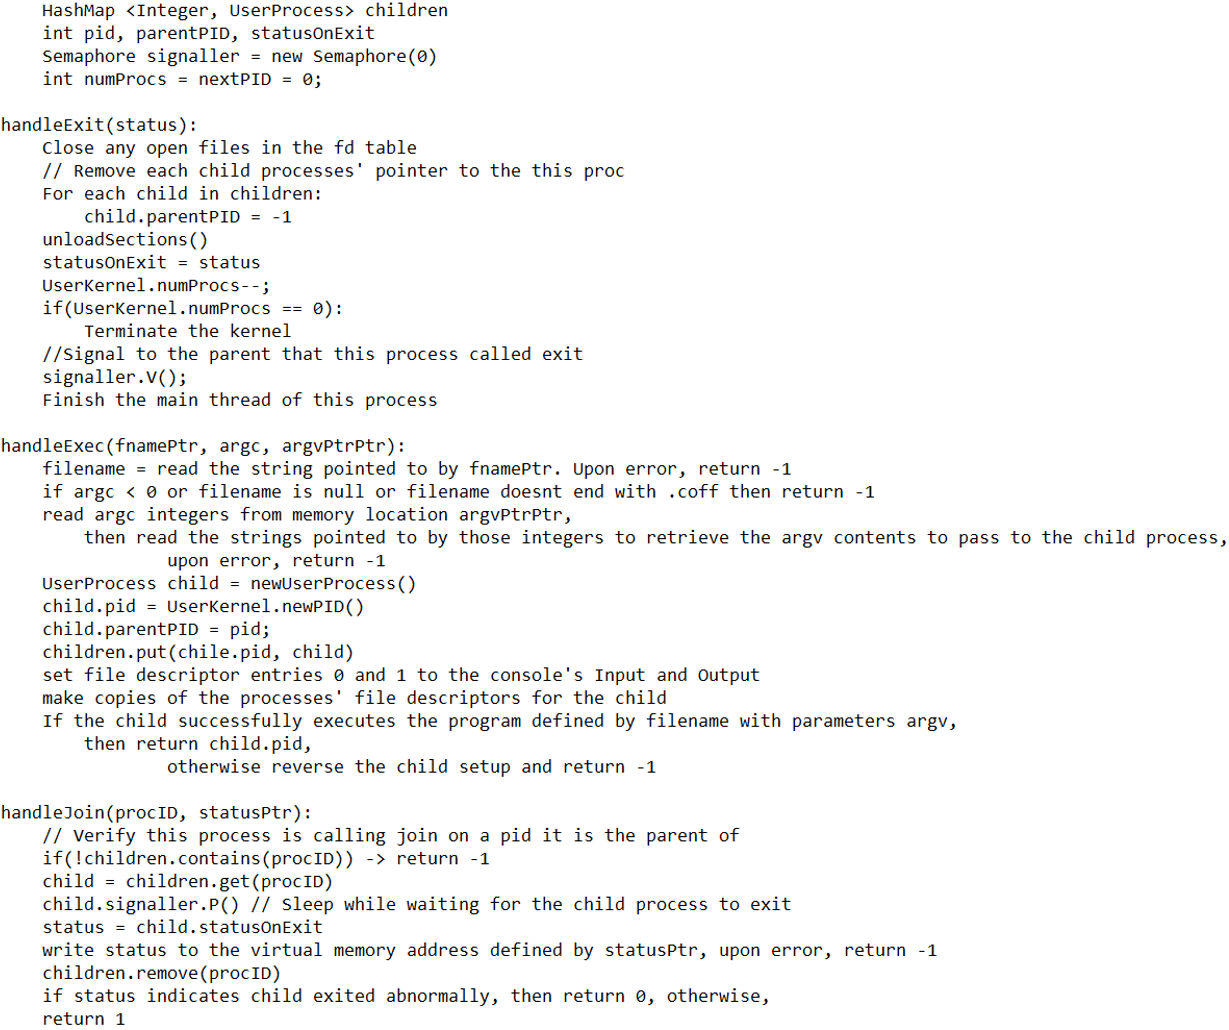
\includegraphics[width=150mm]{pic3_3.png}\end{center}
Where the data structures of \textsc{User Process} and \textsc{User Kernel} are \textsc{HashMap<Integer}, {UserProcess}$>$ \textit{children}\textbf{,} \textsc{int pid}, \textsc{parentPID}, \textsc{statusOnExit}\textbf{,} \textsc{Semaphore} \textit{signaller} = \textit{new} \textsc{Semaphore}(0) 
and \textsc{int numProcs}\textbf{,} \textsc{int nextPID} respectively.
\paragraph{}The \textsc{handleExit} function introduces child process IDs, open file maintenance
data structures, and status variables in conjunction with the de$-$allocation of the 
file descriptor objects. This is done in order to successfully an exit and close all left open files.
In this manner the iteration of the child processes to succeed in the removal of parent pointer 
establishes the \textsc{unloadSection} dependence which provides the successful exiting of the processes.    
\paragraph{}Within the \textsc{handleExec} function are manipulations of the \textsc{argv pointer array} to pass arguments to the new executible. This ensures the that the \textsc{exec} handler would obtain the pointers to the {argv} \textbf{char} buffers and read from \textsc{virtual memory} to achieve execution capabilities. The return is of type \textbf{int} which signifies either an error or under succesful circumstances returns a process ID.
\paragraph{}.
\begin{center}Task IV\end{center}
\paragraph{}Initially, the preliminary idea behind developing a sound and complete implementation of a lottery$-$based scheduler was to change
  the maximum and minimum priority value\textit{d} variables. As such, the lottery scheduler can incorporate its algorithmic
  functionality from the priority queue, respectively. In this manner the lottery scheduler would basically be a priority queue with the 
  maximum value assigned as the highest \textsc{Integer} value available in \textsc{java} and the minimum value being initialized to one 
  representing every thread that receives at least one ticket, therefore the priority will be changed to being reliant on tickets. \\
\paragraph{}From this description it can be gathered that in order to select the thread that \textit{wins} the lottery, first it would go through all
  threads in the queue and add up all the tickets to find total number of tickets in queue (this may be inefficient however, because this 
  would have to be done every time the \textsc{nextThread} function is called). Once this number is found, a random number generator will 
  be used to simulate the lottery with an interval of possibilities from the aforementioned number to the sum of the queue’s tickets. Once 
  this random number is found it would perform iterative computations through the thread queue and distinguish which thread contains that 
  ticket. However To be able to have unique tickets, support threads containing a large amount of tickets, and not keep track of the status 
  of, as a plausible assumption might be, a plethora of tickets (which must consequently be allocated a lot of memory) a methodology of 
  creating unique intervals while finding the sum of queue tickets must be used.\\
\paragraph{}This process is best explained through exemplification. For instance, suppose two threads are in a queue and they each have five tickets; 
  the random number generator would iterate between 1$\longrightarrow$10. Assuming the number 7 is produced from the random number generator,
  each thread would be assigned an interval and the process would begin from top of the queue to the end. Ergo, the top thread would be assigned 
  the interval 1$\longrightarrow$5 to represent it's 5 tickets. In this manner the other thread would be assigned an interval of 
  6$\longrightarrow$10. Therefore, since the second thread has the random number within it's interval, it is the thread that gets selected and 
  removed from the queue. \\\\
The \textsc{nextThread} described below is the new function that would be defined in order for the priority queue to override it in the lottery scheduler and not the \textsc{nextThread} function as defined in the priority scheduler.
\begin{center}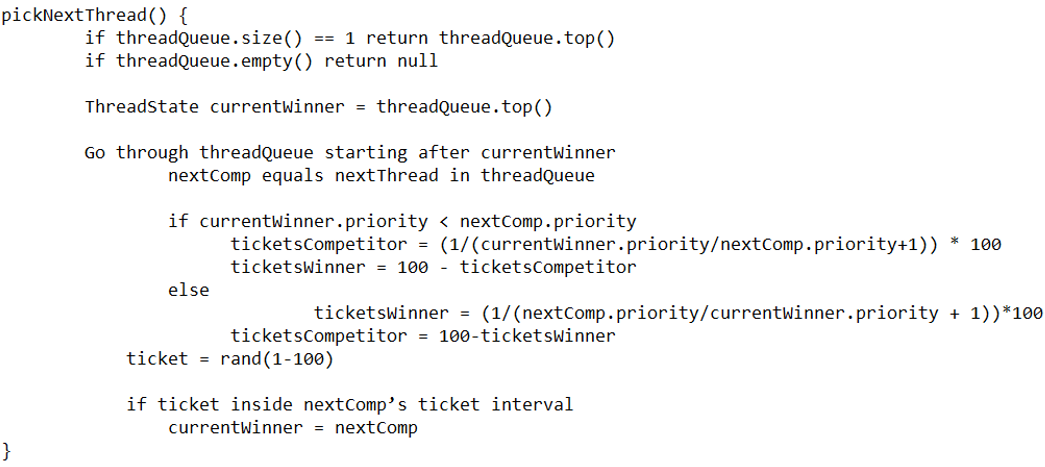
\includegraphics[width=140mm]{pic4_4.png}\end{center}
}
{\setlength{\parindent}{0cm}
\textbf{Design Decisions}
\\\\ \paragraph{}The primary factors of significant importance to the design considerations for the development of a multi$-$programming file system were the scalability, robustness, and efficiency of the system in accordance with the resources 
  associated with its support. In this manner the utilization of data structures, primitive types included, such as priority queues was 
  preeminently regnant to the functionality of the objects defined. For example classes such as \textsc{ticketInterval} were omitted from utilized 
  for the \textsc{LotteryScheduler} class in order to hold a small lottery between two threads and then allow the thread that wins that lottery to go on to have a lottery with the next thread in the queue. 
  Although the \textsc{ticketInterval} class was provided its omission enabled the more efficient functionality of the \textsc{LotteryScheduler} algorithm.
  \\\\
  \paragraph{}Another issue of equal importance is the fact that the virtual memory functionalities of \textbf{Task 2} were changed from the initially proposed implementation
  in order to account for a heap error that became eminent during the execution of the implementation against established corner cases. In this manner the virtual memory was detected to act sporadically and began to allocated
  unprecedented amounts of memory. As such the response to alter the \textsc{read} $\&$ \textsc{write} functions was an integral decision of the design
  process. Therefore, \textsc{readVirtualMemory} was provided checks to not only ensure that the virtual address is valid, but if it isn't to attempt to read one byte at a time from the address in question and assume that it is an invalid address otherwise.
\begin{center}Essentially these design decisions ameliorated the \textbf{Testing/QA} phase of the development endeavor.\end{center}
}
{\setlength{\parindent}{0cm}
\textbf{Testing/QA}\\
\begin{center}Task I\end{center}
In order to establish a testing strategy on the validity of the implementation for the \textsc{read} $\&$ \textsc{write} functions of the first six functions introduced in \textbf{Task 1}, a stress test was performed in which a large chunk of memory was dedicated to \textsc{read} $\&$ \textsc{write} by creating an array that maintains a large number of integers.
In this manner a for loop was then introduced to fill up the array with values and then another for loop to iterate through the array and assert that the values are correctly maintained in order to test that the corresponding sections and pages are functioning correctly.
\begin{center}Task II\end{center}
In order to induce an out of memory error the following test file was used.
\begin{center}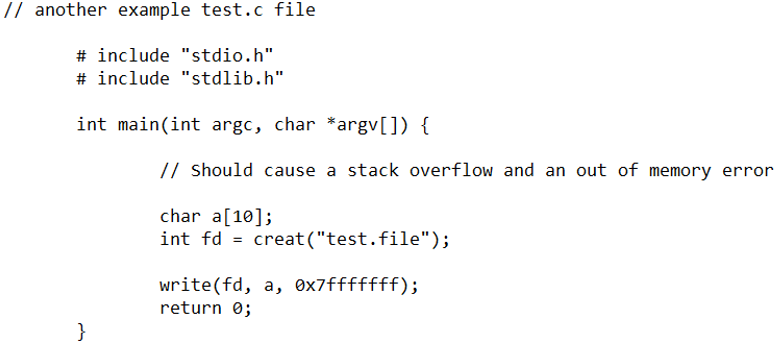
\includegraphics[width=120mm]{test2.png}\end{center}
Through the execution of this source file a stack overflow error was generated and the responsive of the code was tested against induced out of memory exceptions in order 
  to solidify its functionality and develop a more efficient virtual memory.      
\begin{center}Task III\end{center}
An example of a test file constructed to invoke during the writing process of an invalid chuck of memory is demonstrated below.
\begin{center}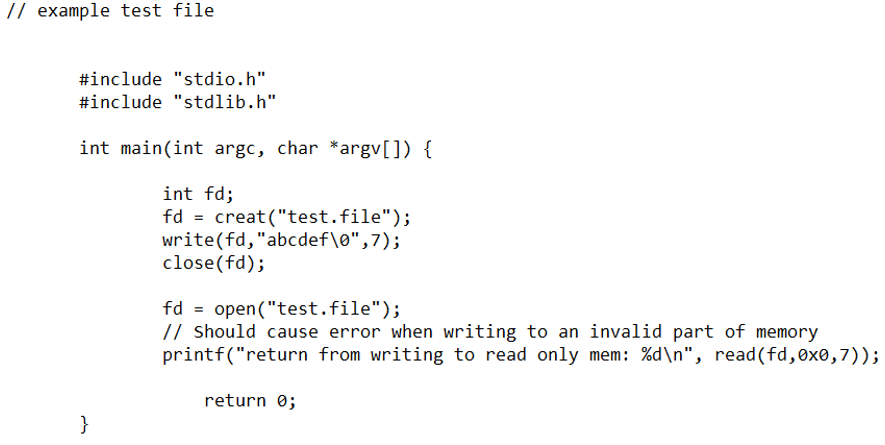
\includegraphics[width=120mm]{test1.png}\end{center}
Within this exemplification, it becomes apparent that there is a copious amount of these lilliputian edge cases/errors. In this manner this becomes paramount to state for the record that this is merely an algorithmic representative   
of many different test cases used to run test cases against the aforementioned implementations. Therefore the test of accessing invalid segments of memory with the intent of writing to read only has passed and served as an integral part of the testing/QA phase of this project. 
\begin{center}Task IV\end{center}
Two main testing strategies were utilized to check for the completeness and correctness of the \textsc{LotteryScheduler} implementation. 
  Firstly, testing on multilevel queues and situations where there were threads with a very large number 
  of tickets was the preliminary method. Testing for multilevel queues was done to make certain that priority 
  donation worked correctly with the addition of tickets to signal priority donation. Testing 
  for tickets with a high amount of tickets was done to make sure that a new system could calculate priorities 
  for threads without needing to compute the sum of all tickets in thread queue.\\\\
}
{\setlength{\parindent}{0cm}
\textbf{Team Member Work-Log}\\ \\
\textbf{\begin{center}\underline{Avery Berchek}\\DevOps Engineer\end{center}} 
\begin{itemize}
\item Designed and outlined the pseudo$-$code for Task III
\item Outlined and participated in the design process associated with Tasks I, II, III, IV
\item Implemented the algorithmic functionality for Task III
\item Primarily responsible for implementation of corner$-$case test cases
\item Conducted and performed code reviews
\item Performed optimizations and ensured the efficiency of the data structures utilized in the source code
\end{itemize}
\textbf{\begin{center}\underline{Aleksandr Brodskiy}\\Project Manager\end{center}}  
\begin{itemize} 
\item Organized the \textit{sprints} and weekly meetings in accordance with the \textit{Agile/Scrum} project management methodology.
\item Delegated tasks and assigned roles for the Engineering Team as well as conducted the code reviews
\item Participated in the design process associated with Tasks I, II, III, IV
\item Created and formatted the Design Documentation
\item Managed all progress and operations of the Engineering Team in order to provide an efficient, robust, and optimal solution for a timely and submission.
\end{itemize}
\textbf{\begin{center}\underline{David Cabral}\\Design Engineer\end{center}} 
\begin{itemize}
\item Designed and outlined the pseudo$-$code for Task IV
\item Implemented the algorithmic functionality for Tasks IV
\item Provided insight and proposed solution for \textit{Lottery Scheduler}
\item Proposed solution and outlined source code structure for Task IV
\end{itemize}
\textbf{\begin{center}\underline{Christopher DeSoto}\\Principal Engineer\end{center}}
\begin{itemize} 
\item Set$-$up the integrated development environment for the entire Engineering Team.
\item Outlined and participated in the design process associated with Task I
\item Implemented the algorithmic functionality for Task I
\item Integrated source code from the \textit{development phase} to the \textit{testing phase} to the \textit{completed phase} to ensure the validity of the solution and provide a general framework for the debugging and testing process for the QA and Software Engineers.
\end{itemize}
\textbf{\begin{center}\underline{Adiam G-Egzabher}\\Systems Engineer\end{center}} 
\begin{itemize}
\item Outlined and participated in the pseudo$-$code development associated with Task I
\item Participated in the design process and Testing/QA phase for Task I
\item Provided insight and proposed solution for Task I 
\end{itemize}
\textbf{\begin{center}\underline{Nanditha Embar}\\QA Engineer\end{center}} 
\begin{itemize}
\item Ensured functionality of all features
\item Provided insight and proposed solution for Task II 
\item Ensured the highest quality attainable with the time and resources provided for submitted source code
\item Participated in the design process and testing/QA phase for Task II
\end{itemize}
\textbf{\begin{center}\underline{Christian Vernikoff}\\Software Engineer\end{center}} 
\begin{itemize}
\item Designed and outlined the pseudo$-$code for Task II
\item Implemented the algorithmic functionality for Tasks II 
\item Outlined and participated in the design process associated with Task II
\end{itemize}
}
{\setlength{\parindent}{0cm}
\textbf{\\\\\\Conclusion}\\ \\
\textit{to be completed upon the final submission of the source code}
\end{document} 
